\chapter{Results and Discussion}
\label{ch:results_and_discussion}



\section{Statistical Evaluation Methodology}
\label{sec:statistical_evaluation_methodology}

\subsection{The Dem\v{s}ar Statistical Framework}
\label{subsec:demsar_framework}

Comparing the performance of multiple forecasting algorithms across a heterogeneous retail portfolio requires rigorous non-parametric statistical testing. This ensures that any observed superiority of a hybrid graph architecture is genuine and not merely the result of stochastic variance or dataset noise. To achieve this, we adopt the widely recognized statistical framework proposed by Dem\v{s}ar (2006) for comparing multiple classifiers over multiple datasets.

Crucially, the statistical evaluation in this study is stratified by the underlying temporal architecture. Rather than pooling all eight models into a single global ranking, the models are divided into two distinct testing pools: LSTM-based architectures (\texttt{lstm\_baseline} and its graph variants) and MLP-based architectures (\texttt{mlp\_baseline} and its graph variants). This isolated comparison guarantees that the statistical tests specifically measure the value added by the topological graph embeddings (GCN, GAT, Graph2Vec) rather than the inherent differences in sequence modeling capabilities between LSTMs and MLPs. The evaluation for each architectural pool is conducted via a two-step process: the omnibus Friedman test followed by the post-hoc Nemenyi test.

\subsubsection{Friedman Omnibus Test}
\label{subsubsec:friedman_test}

The first step of the framework utilizes the Friedman test, a non-parametric equivalent of the repeated-measures ANOVA. Because raw error metrics (such as RMSE) are highly scale-dependent, the Friedman test operates entirely on ranks. For every individual item in the dataset, the models within the respective architectural pool are ranked based on their performance metric, with the best-performing model receiving a rank of 1. 

The test analyzes the average ranks across all items to evaluate the null hypothesis ($H_0$): that all competing models within the pool perform equivalently, and any observed divergence in their average ranks is purely coincidental. If the calculated test statistic results in a p-value below the standard significance threshold ($\alpha = 0.05$), the null hypothesis is rejected, confirming that statistically significant differences exist among the tested models.

\subsubsection{Post-hoc Nemenyi Analysis}
\label{subsubsec:posthoc_nemenyi}

If the Friedman test successfully rejects the null hypothesis, we proceed to the second step: the post-hoc Nemenyi test. This test is designed to identify exactly which specific architectural pairings exhibit significant performance differences while strictly controlling the family-wise error rate associated with multiple comparisons.

The Nemenyi test calculates a Critical Difference (CD) threshold based on the number of models being compared and the total number of datasets (items). The performance of any two models is considered statistically significantly different if, and only if, the absolute difference between their average ranks is equal to or strictly greater than the CD threshold. This highly conservative approach provides mathematically verified proof of whether a proposed graph hybrid genuinely outperforms its standard temporal baseline.

\subsection{Spearman Results and Discussion}
\label{subsec:spearman_results}

This section details the statistical evaluation of the models when constructed using the Spearman rank correlation network threshold. The performance is analyzed by looking at the models' ability to capture the complex temporal dynamics of the retail portfolio, divided by their base architecture.

\subsubsection{LSTM Architectures}
\label{subsubsec:spearman_lstm}

The evaluation of the LSTM-based architectures examines whether injecting structural demand relationships, derived from the Spearman-thresholded similarity graph, benefits recurrent temporal forecasting under the MAE criterion. The Friedman omnibus test yielded a test statistic of $114.05$ ($p = 1.47 \times 10^{-24}$), decisively rejecting the null hypothesis of equal performance and confirming significant differences within the LSTM pool.

Contrary to the expectation that spatial context aids forecasting, the post-hoc Nemenyi analysis reveals that the \texttt{lstm\_baseline} and the macro-level \texttt{graph2vec\_lstm} are the top-performing architectures. The \texttt{lstm\_baseline} attains the lowest average rank of $2.180$, but it is not statistically significantly better than \texttt{graph2vec\_lstm} (rank $2.265$, $p = 0.6645$). Both of these models significantly outperform the localized routing hybrids: \texttt{gcn\_lstm} (rank $2.727$, $p < 0.0001$) and \texttt{gat\_lstm} (rank $2.828$, $p < 0.0001$). This indicates that, under this graph construction, the recurrent encoder already captures the relevant temporal dynamics. While a global macro-embedding does not harm performance, introducing localized node-level spatial signals acts as noise rather than useful context. Attention-weighted aggregation is the most detrimental: \texttt{gat\_lstm} is the worst-ranked model overall. This suggests that the learned spatial attention amplifies, rather than filters, the error introduced by the demand graph. These MAE hierarchies are visualized in the Critical Difference diagram in Figure~\ref{fig:cd_diagram_mae_spearman_lstm}.

\begin{figure}[htbp]
    \centering
     
\includegraphics[width=\linewidth]{figures/cd_diagram_mae_spearman_lstm_total.pdf}
    \caption{Critical Difference (CD) diagram for the LSTM-based architectures evaluated on absolute error (MAE) using the Spearman graph. Models connected by a horizontal bar do not possess statistically significant differences ($\alpha = 0.05$).}
    \label{fig:cd_diagram_mae_spearman_lstm}
\end{figure}

Conversely, while structural embeddings offer no advantage for absolute magnitude forecasting, analyzing the directional accuracy (POCID) reveals a starkly contrasting dynamic. The Friedman omnibus test for POCID yielded a highly significant test statistic of $135.45$ ($p = 3.62 \times 10^{-29}$), confirming profound differences in trend-prediction capabilities among the LSTM variants.

\begin{figure}[ht]
    \centering
     
\includegraphics[width=\linewidth]{figures/cd_diagram_pocid_spearman_lstm_total.pdf}
    \caption{Critical Difference (CD) diagram for the LSTM-based architectures evaluated on directional accuracy (POCID) using the Spearman graph. Higher POCID yields lower ranks.}
    \label{fig:cd_diagram_pocid_spearman_lstm}
\end{figure}


The subsequent Nemenyi analysis demonstrates a complete reversal of the MAE hierarchy: the \texttt{lstm\_baseline} is the worst-performing model for directional accuracy, falling to the highest average rank of $2.908$. When the objective shifts to predicting the correct direction of demand movement, the graph-augmented models systematically outperform the standalone recurrent encoder. The \texttt{gat\_lstm} architecture secures the top rank ($2.112$), followed closely by \texttt{gcn\_lstm} ($2.343$) and \texttt{graph2vec\_lstm} ($2.637$). Notably, even the weakest structural hybrid, \texttt{graph2vec\_lstm}, achieves a statistically significant victory over the baseline ($p = 0.0015$). This fascinating dichotomy indicates that while spatial aggregation introduces variance that harms absolute error, the topological context is highly beneficial for recognizing broader, synchronized market trends and structural inflection points that a purely univariate LSTM fails to anticipate. The statistical tier list for directional accuracy is confirmed in Figure~\ref{fig:cd_diagram_pocid_spearman_lstm}.





\subsubsection{MLP Architectures}
\label{subsubsec:spearman_mlp}

A parallel evaluation was conducted for the MLP-based models to assess the impact of graph embeddings on feed-forward temporal architectures. First, we evaluated the models' forecasting performance under the absolute error criterion (MAE). The Friedman omnibus test confirmed global significance within the MLP pool, yielding a test statistic of $117.84$ ($p = 2.25 \times 10^{-25}$).

Mirroring the dynamic observed in the LSTM evaluation, the addition of structural demand relationships did not improve the magnitude forecasting capabilities of the purely feed-forward architectures. The Nemenyi pairwise comparisons indicate that the \texttt{mlp\_baseline} achieved the lowest (best) average rank of $2.178$. However, it statistically ties with the macro-level \texttt{graph2vec\_mlp} (rank $2.253$, $p = 0.7458$). Both models significantly outperform the localized spatial routing methods: \texttt{gcn\_mlp} (rank $2.757$, $p < 0.0001$) and \texttt{gat\_mlp} (rank $2.812$, $p < 0.0001$). The overarching trend persists: for minimizing absolute deviation, the raw univariate temporal signals are sufficient, and the Spearman-derived node-level spatial context acts primarily as disruptive noise. The complete hierarchy for absolute error is visualized in Figure~\ref{fig:cd_diagram_mae_spearman_mlp}.

However, when evaluating the models on directional accuracy (POCID), the structural embeddings once again demonstrate their value. The Friedman test for POCID across the MLP pool resulted in a highly significant rejection of the null hypothesis (Test Statistic = $38.73$, $p = 1.98 \times 10^{-8}$).

The subsequent post-hoc Nemenyi analysis reveals a reversal of the absolute error hierarchy. When predicting demand trends rather than precise volumes, the localized graph-augmented architectures excel. The \texttt{gat\_mlp} hybrid secures the top rank ($2.343$), closely followed by the \texttt{gcn\_mlp} ($2.357$). Conversely, the standalone \texttt{mlp\_baseline} falls to the worst average rank of $2.731$, being significantly outperformed by the \texttt{gcn\_mlp} architecture ($p < 0.0001$) and its attention-weighted counterpart. The macro-level \texttt{graph2vec\_mlp} embedding bridges the gap between the localized methods and the baseline, achieving a rank of $2.568$.

This consistency across both recurrent (LSTM) and feed-forward (MLP) base architectures provides compelling evidence for the core hypothesis of this research: dynamic graph thresholding captures vital structural market movements and trend inflections that standard univariate models remain blind to. The statistical tier list for directional accuracy is confirmed by the Critical Difference diagram in Figure~\ref{fig:cd_diagram_pocid_spearman_mlp}.

\begin{figure}[htbp]
    \centering
    
\includegraphics[width=\linewidth]{figures/cd_diagram_mae_spearman_mlp_total.pdf}
    \caption{Critical Difference (CD) diagram for the MLP-based architectures evaluated on absolute error (MAE) using the Spearman graph. Models connected by a horizontal bar do not possess statistically significant differences ($\alpha = 0.05$).}
    \label{fig:cd_diagram_mae_spearman_mlp}
\end{figure}

\begin{figure}[htbp]
    \centering
    
\includegraphics[width=\linewidth]{figures/cd_diagram_pocid_spearman_mlp_total.pdf}
    \caption{Critical Difference (CD) diagram for the MLP-based architectures evaluated on directional accuracy (POCID) using the Spearman graph. Higher POCID yields lower ranks.}
    \label{fig:cd_diagram_pocid_spearman_mlp}
\end{figure}


Beyond the rank-based Nemenyi analysis, evaluating the mean percentage change in absolute error (MAE) relative to the \texttt{lstm\_baseline} further quantifies the impact of the structural embeddings. Consistent with the statistical rankings, the integration of spatial context resulted in a consistent degradation of magnitude forecasting accuracy. The macro-level \texttt{graph2vec\_lstm} experienced a minor performance drop of -1.97\%. However, the localized routing methods suffered more substantial penalties, with the \texttt{gcn\_lstm} and \texttt{gat\_lstm} degrading by -2.88\% and -4.99\%, respectively. This quantifiably confirms that for absolute error, node-level spatial aggregation acts as disruptive noise rather than constructive context.

In stark contrast, the mean percentage improvements for directional accuracy (POCID) highlight the distinct advantage of the graph-augmented LSTM models. When shifting the objective to predicting the correct direction of demand movement, the structural hybrids demonstrated clear, quantifiable gains over the baseline. The \texttt{graph2vec\_lstm} achieved a solid +3.66\% improvement. The localized methods leveraged the topological context even more effectively, yielding substantial enhancements: the \texttt{gcn\_lstm} improved by +6.70\%, while the top-ranked \texttt{gat\_lstm} delivered a remarkable +7.93\% increase in trend-prediction accuracy, underlining the power of attention-weighted spatial routing for market inflections.

A parallel dynamic is observed within the feed-forward architectures when evaluating absolute error. The mean percentage change in MAE relative to the \texttt{mlp\_baseline} demonstrates a quantifiable performance degradation across all structural hybrids. The \texttt{graph2vec\_mlp} saw a modest error increase, degrading by -1.83\%. The localized convolutional and attention variants were penalized more heavily, with the \texttt{gat\_mlp} and \texttt{gcn\_mlp} experiencing performance drops of -3.37\% and -3.76\%, respectively. This perfectly mirrors the LSTM dynamics, proving that raw univariate signals are superior for minimizing absolute deviation in purely feed-forward setups.

Finally, examining the mean percentage improvements for MLP directional accuracy (POCID) solidifies the value of spatial routing for trend forecasting. Every graph-augmented variant demonstrated clear gains over the standalone \texttt{mlp\_baseline}. The macro-level \texttt{graph2vec\_mlp} yielded a +1.88\% improvement. More impressively, the localized methods drove significant enhancements in predicting demand direction, with the \texttt{gat\_mlp} improving by +3.80\% and the \texttt{gcn\_mlp} achieving the highest boost at +5.21\%. These percentages reinforce the finding that dynamic graph thresholding is highly effective at capturing synchronized market movements that standard univariate MLPs miss.

\subsection{Product-level Analysis}
The heatmaps presented above reveal considerable heterogeneity across the 60 products: 
graph-augmented hybrids offer meaningful gains for a subset of products, while for 
others the baseline proves difficult to beat.
It is important to note that all comparisons are made on a best-seed basis: for each 
product, the baseline value reported is taken from the seed that minimised its MAE, 
and likewise each hybrid model is represented by its own best-performing seed. 
This seed-selection procedure ensures that every model is evaluated at its strongest, 
avoiding penalising any architecture for unfavourable random initialisations, while 
simultaneously making the comparisons conservative — a hybrid must outperform the 
baseline even under optimal conditions for both.

\subsubsection*{Best-Performing Products}
The heatmaps presented above reveal considerable heterogeneity across the 60 products: 
graph-augmented hybrids offer meaningful gains for a subset of products, while for 
others the baseline proves difficult to beat.
It is important to note that all comparisons are made on a best-seed basis: for each 
product, the baseline value reported is taken from the seed that minimised its MAE, 
and likewise each hybrid model is represented by its own best-performing seed. 
This seed-selection procedure ensures that every model is evaluated at its strongest, 
avoiding penalising any architecture for unfavourable random initialisations, while 
simultaneously making the comparisons conservative — a hybrid must outperform the 
baseline even under optimal conditions for both.
This section highlights the most consistent winners and losers under this evaluation 
protocol.
\textbf{Product 915640} stands out as the product that benefits most from graph 
augmentation in terms of error reduction. Across all three LSTM hybrids the MAE 
improvement over the baseline reaches \(+15.5\%\), \(+20.8\%\), and \(+23.4\%\) 
respectively (Figures~\ref{fig:heatmap_lstm_mae_p1}--\ref{fig:heatmap_lstm_mae_p2}), 
and the MLP family echoes the same pattern with gains of \(+13.0\%\), \(+21.5\%\), 
and \(+20.5\%\) (Figures~\ref{fig:heatmap_mlp_mae_p1}--\ref{fig:heatmap_mlp_mae_p2}). 
The graph signal therefore contributes consistently and substantially for this product 
regardless of the choice of forecaster backbone. The directional accuracy (POCID), 
however, does not follow the same trend — POCID improvements are modest or slightly 
negative for this product (Figures~\ref{fig:heatmap_lstm_pocid_p1}--\ref{fig:heatmap_lstm_pocid_p2}, 
\ref{fig:heatmap_mlp_pocid_p1}--\ref{fig:heatmap_mlp_pocid_p2}) — suggesting that 
the graph embedding helps the model reduce magnitude error without fully correcting 
directional bias.

\textbf{Product 921558} shows reliable MAE gains across both families 
(\(\approx +8\%\) for LSTM, \(\approx +14\%\) for MLP; 
Figures~\ref{fig:heatmap_lstm_mae_p2}, \ref{fig:heatmap_mlp_mae_p2}) and 
simultaneously benefits from strong POCID improvements in the LSTM family 
(\(+7.6\%\) to \(+19.0\%\); Figure~\ref{fig:heatmap_lstm_pocid_p2}), making it 
one of the few products where graph augmentation improves both accuracy metrics 
together under the LSTM backbone.

\textbf{Product 908786} achieves the largest LSTM MAE gains overall (\(+14.0\%\), 
\(+17.2\%\), \(+13.9\%\); Figure~\ref{fig:heatmap_lstm_mae_p2}), with the 
improvement uniformly distributed across all three hybrids, indicating that the 
graph structure rather than a specific architecture is driving the benefit.

\textbf{Product 500056} and \textbf{product 933457} are notable from a directional 
accuracy standpoint: in the LSTM POCID heatmap 
(Figures~\ref{fig:heatmap_lstm_pocid_p1}--\ref{fig:heatmap_lstm_pocid_p2}) both 
products show consistently positive improvements across all three hybrids 
(\(+17.4\%\), \(+20.7\%\), \(+15.2\%\) and \(+3.2\%\), \(+22.3\%\), \(+22.3\%\) 
respectively), suggesting the graph neighbourhood encodes useful directional 
co-movement signals for these products.

\subsubsection*{Worst-Performing Products}

\textbf{Product 26002} is the clearest case of consistent graph-induced degradation. 
In the LSTM MAE heatmap (Figure~\ref{fig:heatmap_lstm_mae_p1}) it records the 
largest negative values in the entire dataset (\(-54.3\%\), \(-28.9\%\), 
\(-54.6\%\)), meaning the hybrid models roughly double the absolute error relative 
to the LSTM baseline. The MLP family shows the same pattern (\(-19.4\%\), 
\(-37.9\%\), \(-46.1\%\); Figure~\ref{fig:heatmap_mlp_mae_p1}). This suggests the 
demand signal for product 26002 carries idiosyncratic dynamics that are poorly 
served — and possibly harmed — by the cross-product graph prior injected via the 
embedding $z$.

\textbf{Product 26220} is the dominant outlier in the MLP family, with MAE 
degradation of \(-28.4\%\), \(-31.2\%\), and \(-25.2\%\) across all three MLP 
hybrids (Figure~\ref{fig:heatmap_mlp_mae_p1}), the most uniformly negative row 
in that heatmap.

\textbf{Product 6032} suffers consistently in both MAE heatmaps 
(LSTM: \(-36.9\%\), \(-12.0\%\), \(-45.9\%\), Figure~\ref{fig:heatmap_lstm_mae_p1}; 
MLP: \(-7.6\%\), \(-15.7\%\), \(-16.5\%\), Figure~\ref{fig:heatmap_mlp_mae_p1}), 
reinforcing the pattern that certain products are structurally incompatible with 
the graph augmentation strategy.


Products that benefit from graph augmentation tend to do so uniformly across all 
three hybrid architectures (Figures~\ref{fig:heatmap_lstm_mae_p1}--\ref{fig:heatmap_mlp_pocid_p2}), 
implying that the improvement is driven by the graph structure itself rather than 
by a particular model design choice. Conversely, products that are harmed also 
suffer across all variants, pointing to a product-level characteristic — such as 
low co-movement with its graph neighbours or a predominantly exogenous demand 
driver not captured by the graph — as the root cause of degradation. Overall, the 
graph signal is beneficial for a minority of products and neutral or harmful for 
the majority, consistent with the aggregate statistics reported in 
Section~\ref{sec:aggregate_results}.

\section{Scalability Analysis}
\label{sec:scalability}

To assess the practical cost of deploying each model at scale, we ran a scalability
benchmark in which every model variant processes a growing number of products
sequentially, from a single product up to $n=500$. For each product we record the
graph construction time (\texttt{build\_s}), the training time (\texttt{train\_s}),
the inference time (\texttt{infer\_s}), and the number of epochs to convergence
(\texttt{epochs\_trained}). Eight variants are compared: two graph-free baselines
(\texttt{lstm\_baseline}, \texttt{mlp\_baseline}) and six graph-based models pairing
each of three neighbourhood encoders (Graph2Vec, GCN, GAT) with an LSTM or an MLP
forecasting head.

% ── Cumulative training cost ─────────────────────────────────────────────
\subsection{Cumulative Training Cost}
\label{sec:scalability-train}

Figure~\ref{fig:cum-train} shows the cumulative training time as the workload grows.
All curves are close to linear in $n$, confirming that per-product training cost is
roughly constant and that no variant exhibits super-linear blow-up as the catalogue
grows. The variants separate into three clear tiers. The graph-free baselines are the
cheapest by a wide margin ($\approx 7{,}000$\,s for the full $500$ products, i.e.
$\approx 14$\,s per product). The Graph2Vec and GCN variants form a middle tier
($\approx 22{,}000$--$40{,}000$\,s). The GAT variants are the most expensive, with
\texttt{gat\_mlp} reaching $\approx 82{,}000$\,s and \texttt{gat\_lstm}
$\approx 62{,}000$\,s, roughly an order of magnitude above the baselines. The
attention mechanism therefore dominates the training budget. The visible ``steps'' in
the curves correspond to individual products that required substantially more epochs
before early stopping triggered.

\begin{figure}[ht]
    \centering
    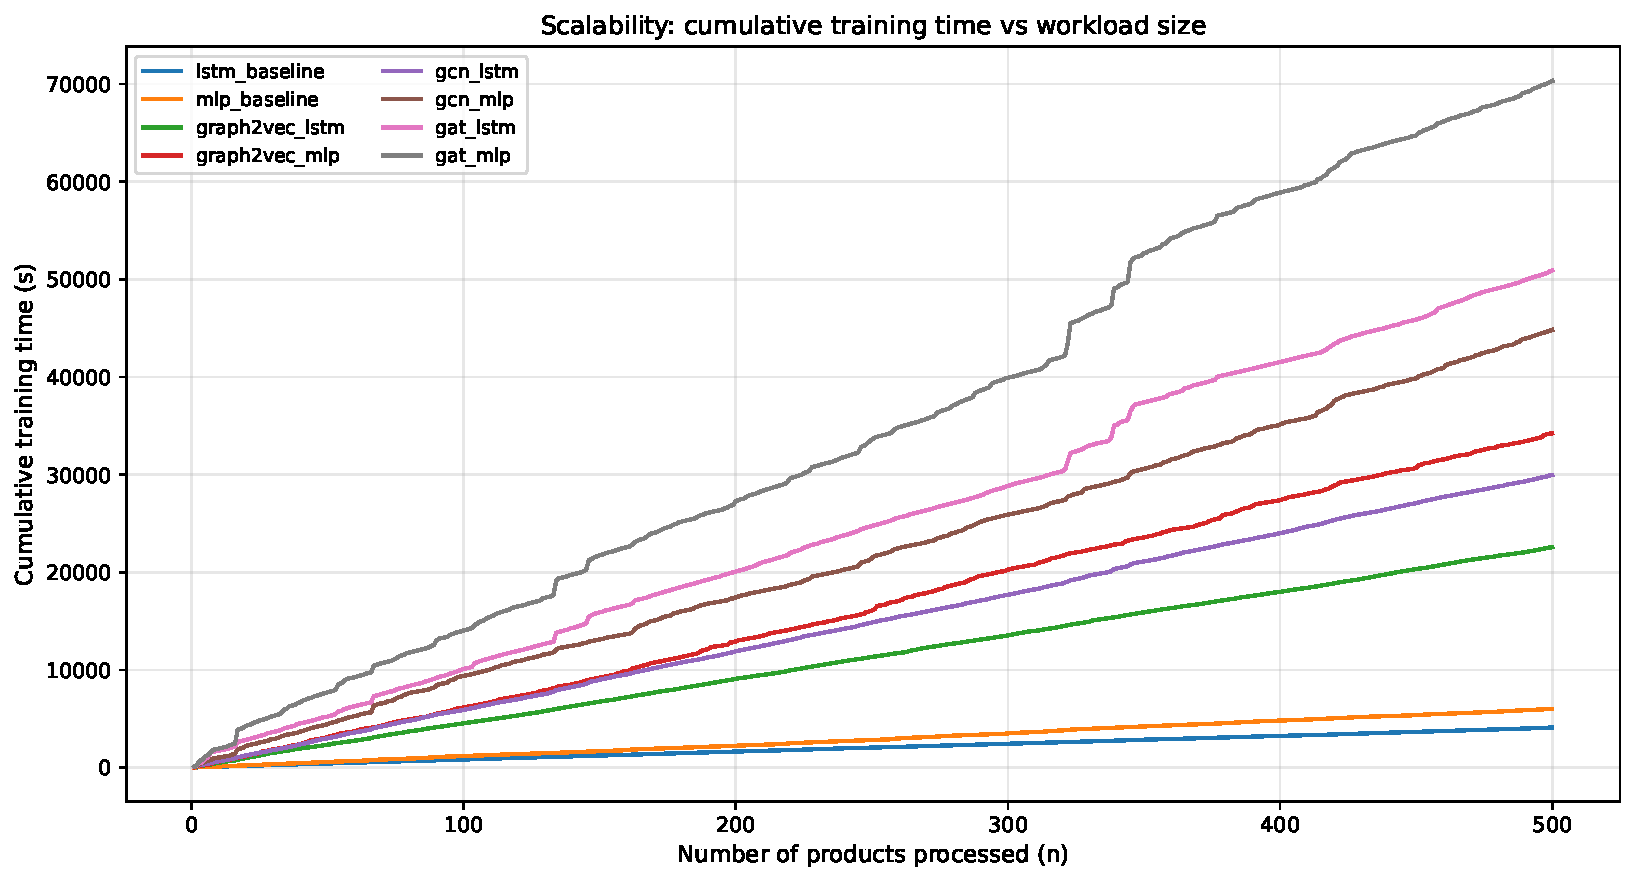
\includegraphics[width=0.7\linewidth]{cum_train_evolution.pdf}
    \caption{Cumulative training time as a function of the number of products
    processed ($n$), one line per model variant. The near-linear growth indicates
    constant per-product cost; the GAT variants are roughly an order of magnitude
    more expensive to train than the graph-free baselines.}
    \label{fig:cum-train}
\end{figure}

% ── Graph construction overhead ──────────────────────────────────────────
\subsection{Graph Construction Overhead}
\label{sec:scalability-build}

Graph construction is a one-off per-product cost shared by all graph-based variants
and absent (zero) for the baselines. Across the graph models the mean build time is
modest and comparable ($\approx 2.1$--$2.9$\,s per product), and it is independent of
the forecasting head. It is therefore not a scalability bottleneck: graph
construction accounts for only a small fraction of the end-to-end cost, which is
dominated by training (Section~\ref{sec:scalability-train}).

% ── Inference cost ───────────────────────────────────────────────────────
\subsection{Inference Cost}
\label{sec:scalability-infer}

Cumulative inference time (Figure~\ref{fig:cum-infer}) again grows linearly in $n$,
but the ordering differs markedly from training. Here the Graph2Vec variants are the
most expensive at inference time --- \texttt{graph2vec\_lstm} reaches $\approx 440$\,s
and \texttt{graph2vec\_mlp} $\approx 275$\,s. It is important to note that all
graph-based variants rebuild the ego-graph from scratch at every forecast step (with
the target node set to the model's own rolling predictions and the neighbours
observed); this rebuild cost is therefore common to all of them. What sets Graph2Vec
apart is that each rebuilt graph must additionally be \emph{re-embedded} by the
trained model --- a Weisfeiler--Lehman relabelling followed by a Doc2Vec
\texttt{infer\_vector} pass --- at every step, whereas the GCN and GAT variants require
only a single forward pass over the rebuilt graph. Consequently the GAT and GCN
variants are cheaper at inference ($\approx 100$--$220$\,s) despite being costlier to
train, and the baselines remain negligible ($\approx 33$\,s). This decoupling of
training and inference cost is relevant for deployment: a model that is expensive to
train once may still be cheap to serve repeatedly, and vice versa.

\begin{figure}[ht]
    \centering
    
\includegraphics[width=0.7\linewidth]{figures/cum_infer_evolution.pdf}
    \caption{Cumulative inference time as a function of the number of products
    processed ($n$), one line per model variant. All graph-based variants rebuild the
    ego-graph at every forecast step; the Graph2Vec variants are nonetheless the most
    expensive because each rebuilt graph must additionally be re-embedded by the
    trained model (Weisfeiler--Lehman relabelling followed by a Doc2Vec
    \texttt{infer\_vector} pass) at every step, whereas the GCN/GAT variants require
    only a single GNN forward pass.}
    \label{fig:cum-infer}
\end{figure}


% ── Training efficiency: epochs and per-epoch cost ───────────────────────
\subsection{Training Efficiency: Epochs and Per-Epoch Cost}
\label{sec:scalability-epochs}

To separate \emph{how many} optimisation steps each model needs from \emph{how
expensive} each step is, Table~\ref{tab:scalability-epochs} reports the mean number of
epochs required to fit one product and the average wall-clock time per epoch.
The mean epoch count is broadly similar across variants ($\approx 125$--$197$), so the
large training-cost differences observed in Section~\ref{sec:scalability-train} are
driven primarily by the per-epoch cost rather than by slower convergence. The
graph-free baselines cost $\approx 0.04$\,s/epoch, the Graph2Vec variants
$\approx 0.28$\,s/epoch (an order of magnitude more), and the GCN/GAT variants more
still. The high standard deviation in epoch counts (e.g. \texttt{graph2vec\_mlp})
reflects the per-product variability of early stopping. Figure~\ref{fig:epochs-analysis}
visualises both quantities side by side.

\begin{table}[ht]
\centering
\caption{Per-model training efficiency: mean number of epochs to fit one product
(with standard deviation) and mean wall-clock time per epoch, averaged over the
$N$ benchmarked products.}
\label{tab:scalability-epochs}
\begin{tabular}{lrrrr}
\toprule
Model variant            & Mean epochs & Std    & Avg. s/epoch & $N$ \\
\midrule
\texttt{lstm\_baseline}  & 146.1       & 58.2   & 0.042        & 500 \\
\texttt{mlp\_baseline}   & 154.8       & 91.6   & 0.039        & 500 \\
\texttt{graph2vec\_lstm} & 137.1       & 37.5   & 0.284        & 500 \\
\texttt{graph2vec\_mlp}  & 197.3       & 135.0  & 0.288        & 500 \\
\texttt{gcn\_lstm}       & 125.1       & 22.1   & 1.052        & 84\textsuperscript{\dag} \\
\texttt{gcn\_mlp}        & ---         & ---    & ---          & --- \\
\texttt{gat\_lstm}       & ---         & ---    & ---          & --- \\
\texttt{gat\_mlp}        & ---         & ---    & ---          & --- \\
\bottomrule
\end{tabular}

\vspace{0.5em}
{\footnotesize \textsuperscript{\dag}\,\texttt{gcn\_lstm} figures are from a partial
run of $84$ products. Dashes denote variants not yet benchmarked for epoch-level
timing.}
\end{table}

\begin{figure}[ht]
    \centering
    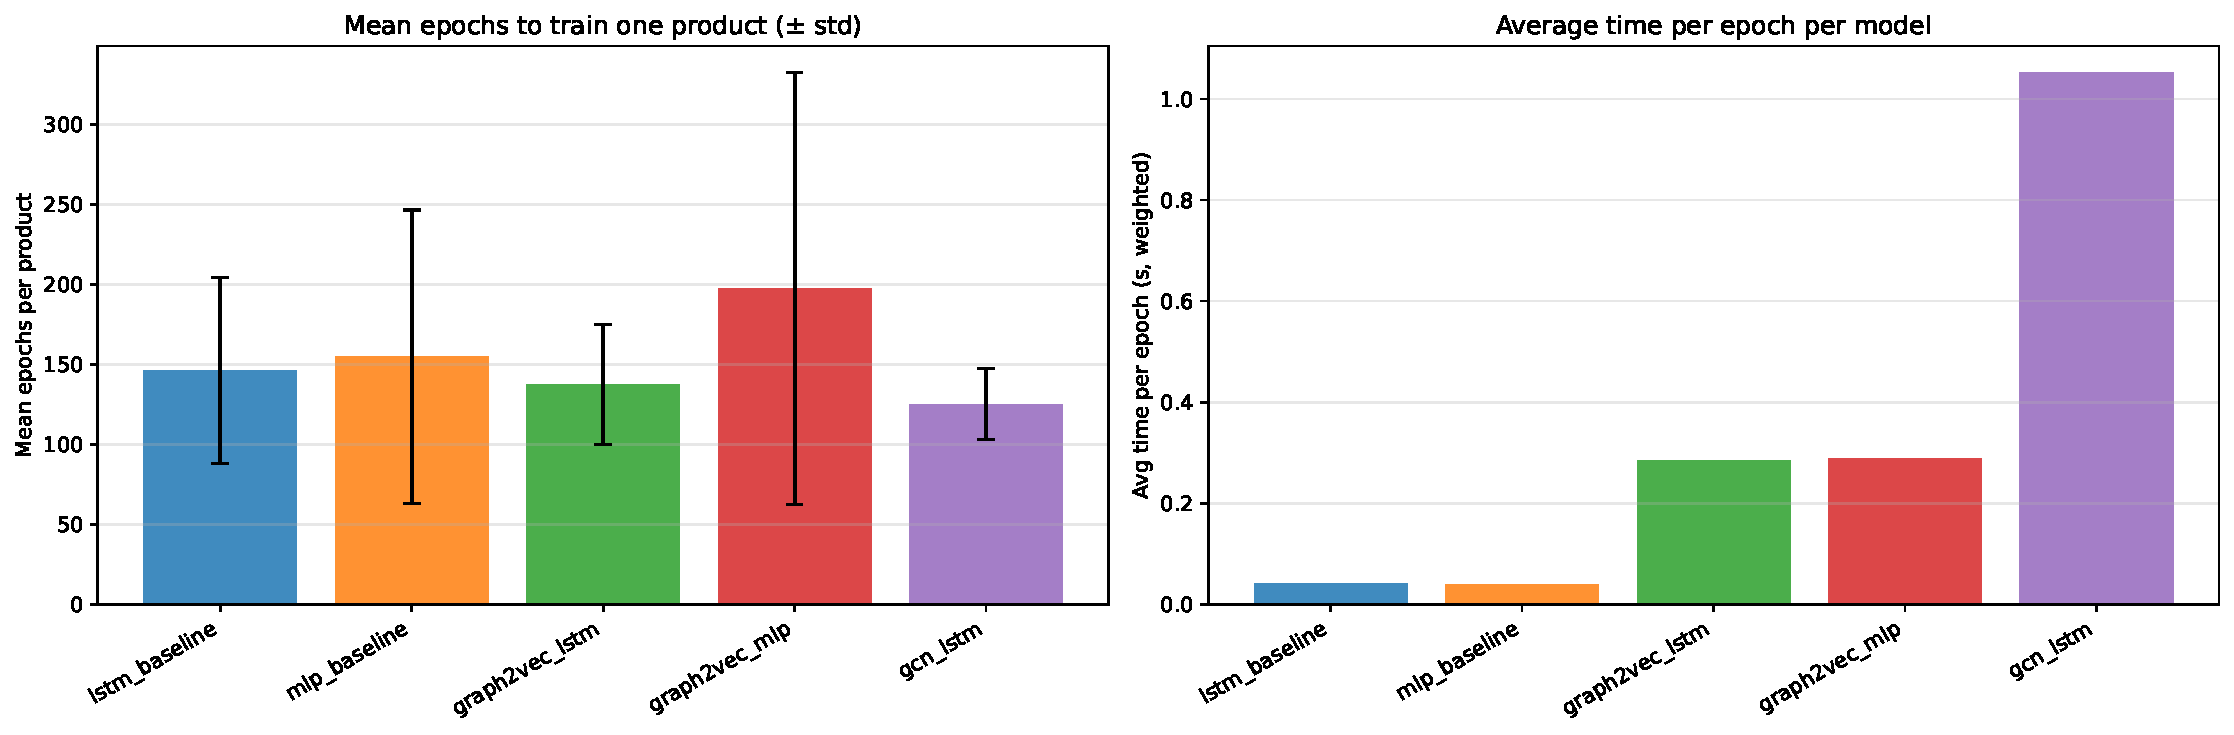
\includegraphics[width=0.7\linewidth]{epochs_analysis.pdf}
    \caption{Left: mean number of epochs to train one product per variant (with
    standard deviation). Right: average wall-clock time per epoch per variant. Epoch
    counts are comparable across variants, so per-epoch cost is the main driver of the
    training-time differences in Figure~\ref{fig:cum-train}.}
    \label{fig:epochs-analysis}
\end{figure}

